\documentclass{article}
\usepackage{graphicx} % Required for inserting images
\usepackage{amsmath} 
\usepackage{tikz}
\usepackage{pgfplots}
\usepackage{xcolor} % Required for colored text

\title{Example for LaTeX}
\author{Aaditya Neupane}
\date{30.07.2024}

\begin{document}

\maketitle

\section{Introduction}
Using LaTeX to Create Math formulas, referencing, drawing, writing \\ presentations.



\section{Some Basic Math Formulas}
\begin{enumerate}
    \item \textbf{Quadratic Formula} $ax^2+bx+c$
    $$ x = \frac{-b \pm \sqrt{b^2 - 4ac}}{2a} $$
    \item \textbf{Area of a Circle}
    $$A = \pi r^2$$
    \item \textbf{Trigonometric Formulas}
    \begin{table}[h]
        \centering
        \begin{tabular}{c|c}
        
            \(\sin(\theta) = \frac{\text{opposite}}{\text{hypotenuse}}\) & \(\csc(\theta) = \frac{\text{hypotenuse}}{\text{opposite}}\)  \\ \\ \hline \\
            \(\cos(\theta) = \frac{\text{adjacent}}{\text{hypotenuse}}\) & \(\sec(\theta) = \frac{\text{hypotenuse}}{\text{adjacent}}\) \\ \\ \hline \\
            \(\tan(\theta) = \frac{\text{opposite}}{\text{adjacent}}\) & \(\cot(\theta) = \frac{\text{adjacent}}{\text{opposite}}\) \\
        \end{tabular}
        \caption{Trigonometric Formulas}
    \end{table}
\end{enumerate}
\section {Integration and Differentiation}
\begin {enumerate}
    \item \textbf{Integrals}
    $$\int_a^b f(x) \, dx = F(b) - F(a)$$
    \item \textbf{Partial Derivative}
     \\Example of a partial derivative equation: For the equation:
     \\\( f(x, y) = x^2 y + y^3 \).
     \\Derivative of \( f \) with respect to \( x \) is:
    \begin{equation}\frac{\partial f}{\partial x} = 2xy\end{equation}
    
    Derivative of \( f \) with respect to \( y \) is:

    \begin{equation}\frac{\partial f}{\partial y} = x^2 + 3y^2\end{equation}
    % \item Area of a Circle
    % $$A = \pi r^2$$
    \item \textbf{Example} of Gradient Descent with scatter points in 3D 
    \\
    \textcolor{gray}{** This image was uploaded, not made using LaTeX **}
    \\
    \includegraphics[scale=0.5]{download.png}
\end {enumerate}


\section {Vector and Matrix}
\begin {enumerate}
 \item \textbf{Vector}
 \\ $$\vec{A}=\vec{B} + \vec{C}$$
 \\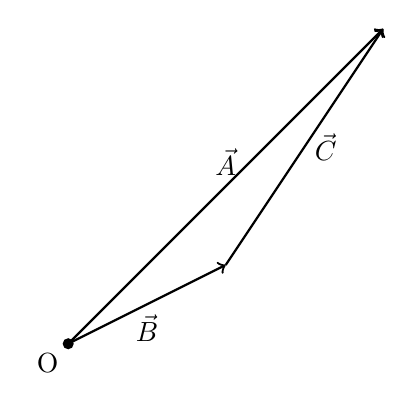
\begin{tikzpicture}
    \draw[->, thick] (0,0) -- (2,1) node[midway, below] {$\vec{B}$};
    \draw[->, thick] (2,1) -- (4,4) node[midway, right] {$\vec{C}$};
    \draw[->, thick] (0,0) -- (4,4) node[midway, above] {$\vec{A}$};
    \fill (0,0) circle (2pt) node[below left] {O};
\end{tikzpicture}
\item \textbf{Matrix}
\\ Example of a 3x3 Matrix:
$$\begin{bmatrix}
    1&2&3
    \\4&5&6
    \\7&8&9
\end{bmatrix}$$
\\
\end {enumerate}

\section{Sin and Cos function Graphs}
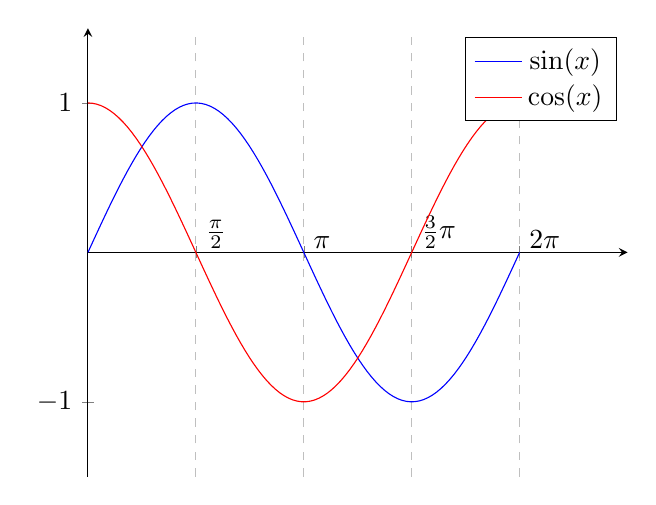
\begin{tikzpicture}
    \begin{axis}[
        clip=false,
        xmin=0,
        xmax=2.5*pi,
        ymin=-1.5,
        ymax=1.5,
        xtick={0,pi/2,pi,3*pi/2,2*pi},
        xticklabels={$0$,$\frac{\pi}{2}$,$\pi$,$\frac{3}{2}\pi$,$2\pi$},
        axis lines = middle,
        xticklabel style={anchor=south west},
        xmajorgrids=true,
        grid style=dashed
    ]
    \addplot[
        domain = 0:2*pi,
        samples = 100,
        color = blue,
    ]{sin(deg(x))};
    \addlegendentry{$\sin(x)$}
    
    \addplot[
        domain = 0:2*pi,
        samples = 100,
        color = red,
    ]{cos(deg(x))};
    \addlegendentry{$\cos(x)$}
    \end{axis}
\end{tikzpicture}


\end{document}
